% File: solutions/ex10.tex

\begin{soluzione}{10}
    Questo esercizio analizza il campionamento di un segnale modulato, dove lo spettro non è centrato sull'origine.

    \subsubsection*{1. Spettro del Segnale Originale, $X(f)$}
    Il segnale è un prodotto nel tempo: $x(t) = g(t) \cdot c(t)$, dove:
    \begin{itemize}
        \item $g(t) = \text{sinc}(4t)$. La sua trasformata è $G(f) = \frac{1}{4}\text{rect}\left(\frac{f}{4}\right)$. Questo è un rettangolo di altezza $1/4$ che si estende da $-2$ Hz a $2$ Hz.
        \item $c(t) = \cos(2\pi \cdot 20t)$. La sua trasformata è $C(f) = \frac{1}{2}[\delta(f-20) + \delta(f+20)]$.
    \end{itemize}
    La trasformata del prodotto è la convoluzione delle trasformate:
    \[
        X(f) = G(f) * C(f) = \frac{1}{2}G(f) * [\delta(f-20) + \delta(f+20)]
    \]
    La convoluzione con gli impulsi di Dirac sposta una copia di $\frac{1}{2}G(f)$ a $+20$ Hz e un'altra a $-20$ Hz. L'ampiezza di queste copie sarà $\frac{1}{2} \cdot \frac{1}{4} = \frac{1}{8}$.
    
    Lo spettro $X(f)$ è quindi composto da due rettangoli:
    \begin{itemize}
        \item Uno centrato a $+20$ Hz, che si estende da $20-2=18$ Hz a $20+2=22$ Hz.
        \item Uno centrato a $-20$ Hz, che si estende da $-20-2=-22$ Hz a $-20+2=-18$ Hz.
    \end{itemize}
    La massima frequenza del segnale è $B = 22$ Hz.

    \begin{center}
    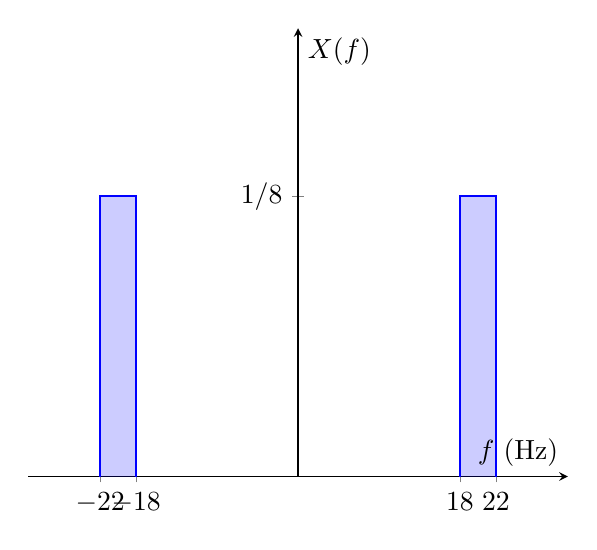
\begin{tikzpicture}
        \begin{axis}[
            axis lines=middle, xlabel=$f$ (Hz), ylabel=$X(f)$,
            xmin=-30, xmax=30, ymin=0, ymax=0.2,
            xtick={-22, -18, 0, 18, 22}, ytick={0.125},
            yticklabels={$1/8$}
        ]
        \addplot[blue, thick, fill=blue, fill opacity=0.2] coordinates {(-22,0) (-22, 0.125) (-18, 0.125) (-18,0)};
        \addplot[blue, thick, fill=blue, fill opacity=0.2] coordinates {(18,0) (18, 0.125) (22, 0.125) (22,0)};
        \end{axis}
    \end{tikzpicture}
    \end{center}

    \subsubsection*{2. e 3. Spettro Campionato e Aliasing}
    Il segnale viene campionato con $f_s = 38$ Hz. L'intervallo di Nyquist è $[-f_s/2, f_s/2] = [-19, 19]$ Hz. Poiché $B=22$ Hz, che è maggiore di $19$ Hz, si verificherà aliasing.
    
    Lo spettro campionato $\tilde{X}(f)$ è una somma di repliche di $X(f)$ scalate di $1/T=f_s=38$. L'ampiezza di ogni rettangolo replicato sarà $\frac{1}{8} \cdot 38 = \frac{19}{4} = 4.75$.
    
    Analizziamo le repliche che cadono (anche parzialmente) nella banda $[-25, 25]$ Hz:
    \begin{itemize}
        \item \textbf{Replica centrale (k=0):} Copie di $X(f)$ centrate a $\pm 20$ Hz.
            \begin{itemize}
                \item Parte positiva: rettangolo da $[18, 22]$ Hz.
                \item Parte negativa: rettangolo da $[-22, -18]$ Hz.
            \end{itemize}
        \item \textbf{Replica di sinistra (k=-1):} Copie di $X(f)$ spostate a sinistra di $f_s$. I centri originali $\pm 20$ Hz si spostano a $\pm 20 - 38$ Hz.
            \begin{itemize}
                \item Centro a $20 - 38 = \mathbf{-18}$ Hz. Produce un rettangolo da $[-20, -16]$ Hz.
                \item Centro a $-20-38 = -58$ Hz (fuori dal nostro grafico).
            \end{itemize}
        \item \textbf{Replica di destra (k=1):} Copie di $X(f)$ spostate a destra di $f_s$. I centri originali $\pm 20$ Hz si spostano a $\pm 20 + 38$ Hz.
            \begin{itemize}
                \item Centro a $-20 + 38 = \mathbf{18}$ Hz. Produce un rettangolo da $[16, 20]$ Hz.
                \item Centro a $20+38 = 58$ Hz (fuori dal nostro grafico).
            \end{itemize}
    \end{itemize}
    Il grafico seguente mostra queste componenti. La replica centrale è in blu, mentre le repliche "aliased" (che si ripiegano nella banda base) sono in rosso.
    
    \begin{center}
    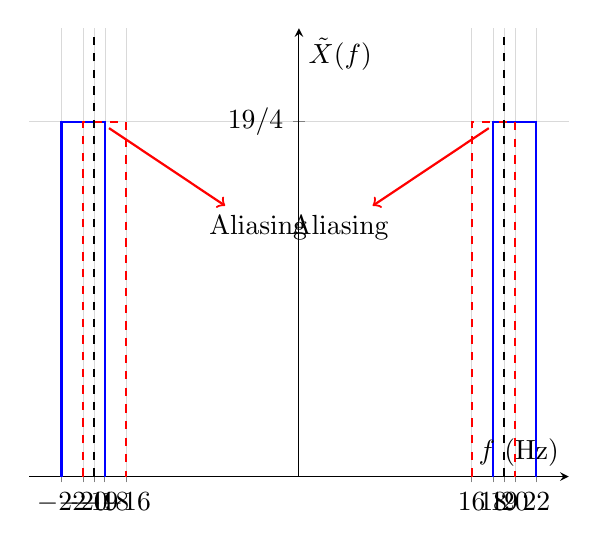
\begin{tikzpicture}
        \begin{axis}[
            axis lines=middle, xlabel=$f$ (Hz), ylabel=$\tilde{X}(f)$,
            xmin=-25, xmax=25, ymin=0, ymax=6,
            xtick={-22, -20, -19, -18, -16, 0, 16, 18, 19, 20, 22},
            ytick={4.75}, yticklabels={$19/4$},
            grid=both, grid style={line width=.1pt, draw=gray!30},
        ]
        % Componenti della replica centrale (k=0)
        \addplot[blue, thick] coordinates {(-22,0) (-22, 4.75) (-18, 4.75) (-18,0)};
        \addplot[blue, thick] coordinates {(18,0) (18, 4.75) (22, 4.75) (22,0)};
        
        % Componenti aliased (k=-1 e k=1)
        \addplot[red, thick, dashed] coordinates {(-20,0) (-20, 4.75) (-16, 4.75) (-16,0)};
        \addplot[red, thick, dashed] coordinates {(16,0) (16, 4.75) (20, 4.75) (20,0)};
        
        % Linee guida per la banda di Nyquist
        \draw[dashed, black, thick] (axis cs:-19, 0) -- (axis cs:-19, 6) node[above, font=\tiny]{$-f_s/2$};
        \draw[dashed, black, thick] (axis cs:19, 0) -- (axis cs:19, 6) node[above, font=\tiny]{$f_s/2$};
        
        \node[pin={[pin edge={red, thick,->}, pin distance=1.5cm]220:{Aliasing}}] at (axis cs:18.5,4.75) {};
        \node[pin={[pin edge={red, thick,->}, pin distance=1.5cm]320:{Aliasing}}] at (axis cs:-18.5,4.75) {};
        
        \end{axis}
    \end{tikzpicture}
    \end{center}
    Come si vede, la replica centrata a $-18$ Hz (rossa) si sovrappone con la replica centrata a $-20$ Hz (blu). Lo stesso accade dal lato positivo. L'aliasing è questa sovrapposizione: la parte della banda originale (blu) che cade fuori dall'intervallo di Nyquist $[-19, 19]$ Hz è indistinguibile dalla parte della replica adiacente (rossa) che cade all'interno.
\end{soluzione}